\capitulo{4}{Técnicas y herramientas}

En este capítulo se exponen todas las herramientas que se han utilizado y las técnicas que se han seguido para poder desarrollar el proyecto de una manera sencilla y organizada. 

\section{Técnicas: metodologías ágiles } \label{sec:HMetodologiasAgiles}
Como metodología ágil \cite{MetodologiasAgiles} para el desarrollo y organización del proyecto, se ha utilizado la metodología SCRUM, ya que además de ser la más usada en el entorno laboral real, ha sido una de las que hemos trabajado durante las asignaturas del grado. Pero para poder entender su potencial veamos que es SCRUM.

SCRUM es un proceso en el que se aplican un conjunto de buenas prácticas que permiten trabajar de forma colaborativa y organizada mediante el uso de Sprint y tareas. 
El desarrollo de todo el proyecto se separa en diferentes Sprint, que contienen una serie de tareas necesarias para conseguir un software final. Cada uno de los Sprint debe ser completado en unas 3 semanas por lo que en la reunión inicial, se deben discutir que tareas estarán en el sprint actual. El equipo deberá valorar la dificultad y el tiempo de cada una de las tareas y tratar de realizar la mayoría de las tareas posibles en ese sprint. En la finalización de cada sprint se deberá entregar un resultado válido. 
En la metodología SCRUM, es de gran importancia la comunicación con el resto del equipo, por lo que al final de cada día se realiza una reunión de unos 15 minutos en la que se exponen problemas, avances y dificultades. En la Figura \ref{diagSrum} encontramos un diagrama que sirve como resumen del funcionamiento de esta técnica.


%\imagen{SCRUM}{Diagrama resumen de la Metodología SCRUM. \cite{SCRUM}} \label{diagSrum}
\begin{figure}[!h]
	\centering
	\includegraphics[width=0.9\textwidth]{SCRUM}
	\caption{Diagrama resumen de la Metodología SCRUM. \cite{SCRUM}}\label{diagSrum}
\end{figure}

Las figuras más importantes de esta metodología son:
\begin{description}
\item[El Product Owner] Es el encargado de hablar con el cliente y exponer sus peticiones al SCRUM master y al equipo de desarrollo. En otras palabras, es quien define las tareas, condiciones y prioridades centrándose en el retorno sobre la inversión, en ingles Return on Investement(ROI), del proyecto.
\item[El SCRUM Master] Es quien dirige y lidera al SCRUM team. Es el encargado de guiar al equipo y hacer que se cumplan las normas de la metodología SCRUM. Esta figura está muy ligada al Product Owner, ayudándole a maximizar el ROI.
\item[El SCRUM team] Es el equipo desarrollador del software del proyecto. Suele estar formado por grupos de entre 3 y 9 personas que deben tener buenas capacidades referidas a la organización y gestión de tareas y procesos.
\end{description}

Partiendo de los actores anteriores podemos definir que, tanto el cargo de Product Owner y SCRUM Team han sido interpretados por mí, a diferencia de la figura de SCRUM Master la habrían representado mis tutores.

Todo esto nos ayuda a poder lograr un resultado final óptimo en el desarrollo de proyectos complejos, dónde se necesita obtener resultados en un corto margen de tiempo y donde las tareas pueden variar. Se usa en entornos complejos donde prima la competitividad, la flexibilidad y la productividad.


\section{Herramientas hardware}\label{sec:HHardware}

Veamos con más detalle los componentes hardware de este proyecto.

\subsection{Placa FRDM K64F}
Esta placa es un conjunto hardware que, además de contener el microcontrolador, nos ofrece las características necesarias para poder conectar varios periféricos a este controlador.

\begin{figure}[!h]
	\centering
	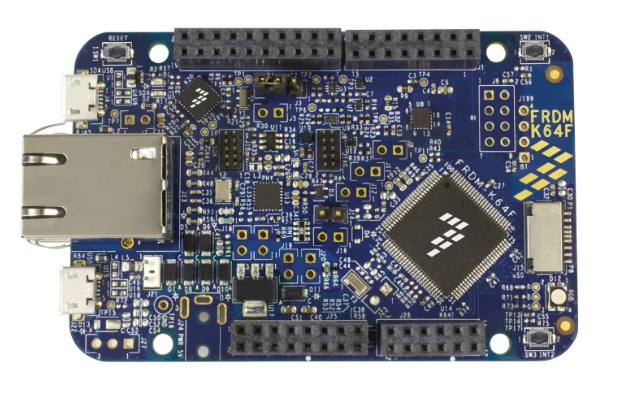
\includegraphics[width=0.7\textwidth]{placa}
	\caption{Placa FRDM K64F.}
\end{figure}
\FloatBarrier

Sus características son:
\begin{itemize}
\item Microcontrolador MK64FN1M0VLL12 MCU: (120 MHz, 1 MB de memoria flash, 256 KB RAM, USB de bajo consumo, sin cristal, y 100 Low profile Quad Flat (LQFP))
\item Núcleo ARM Cortex M4F. \cite{Cortex}
\item Interfaz USB de doble función con conector USB micro-B
\item LED RGB
\item Acelerómetro y magnetómetro FXOS8700CQ
\item Dos botones de usuario
\item Opción de alimentación flexible - OpenSDAv2 USB, Kinetis K64 USB y fuente externa
\item Fácil acceso a la entrada/salida del MCU a través de Arduino™ R3 compatible Conectores de E/S
\item Circuito de depuración programable OpenSDAv2 compatible con el software CMSISDAP Interface que proporciona:
\begin{itemize}
\item Interfaz de programación flash del dispositivo de almacenamiento masivo (MSD)
\item Interfaz de depuración CMSIS-DAP a través de una conexión USB HID sin controlador proporcionando depuración de control de ejecución y compatibilidad con herramientas IDE
\item Interfaz de puerto serie virtual
\item Proyecto de software CMSIS-DAP de código abierto
\item Ethernet
\item SDHC
\item Módulo RF adicional: nRF24L01+ Nordic 2.4GHz Radio
\item Módulo Bluetooth adicional: JY-MCU BT board V1.05 BT
\end{itemize}
\end{itemize}
 

Se puede encontrar más información acerca de los microcontroladores en el libro: \cite{Freescale}.

\subsection{Placa de expansión Arduino Basic I/O}

\begin{figure}[!h]
	\centering
	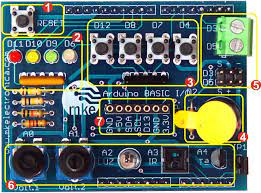
\includegraphics[width=0.6\textwidth]{shield}
	\caption{Placa de expansión Arduino basic I/O.}
\end{figure}
\FloatBarrier

Esta placa se sitúa sobre la placa K64F conectándola directamente sobre sus pines y dotándola de varias características, como por ejemplo:
Altavoz, 4 leds de diferentes colores, 4 botones, sensor de infrarrojos, 2 potenciómetros, entre otros. De esta manera se consigue dotar a la placa de más funciones.

\subsection{LCD}

Una pantalla LCD (\extranjerismo{liquid crystal display)} o pantalla de cristal líquido, es una pantalla delgada y plana. Puede estar formada por píxeles monócromos o en color, colocados sobre una fuente de luz. Estos píxeles son una capa de moléculas situada entre dos electrodos transparentes, dos filtros polarizados. Sin cristal líquido entre el filtro polarizante, la luz quedaría bloqueada al tratar de pasar el segundo filtro.

\begin{figure}[!h]
 \centering
  \subfloat[Pantalla LCD]{
    \includegraphics[width=0.5\textwidth]{PantallaLCD.png}}
  \subfloat[Modulo IIC/I2C]{
    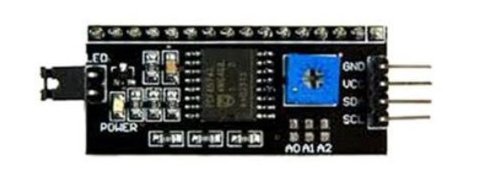
\includegraphics[width=0.5\textwidth]{moduloLCD.png}}
 \caption{Pantalla LCD con modulo IIC/I2C.}
 \label{f:animales}
\end{figure}

Tanto para el desarrollador como sobre todo para el cliente final que recibe el proyecto, es interesante el uso de una pantalla que muestre información sobre las operaciones que está realizando el sistema empotrado. En este proyecto, se ha utilizado una pantalla de 2 líneas de 16 caracteres cada línea. Por lo general, estas pantallas necesitan de la conexión de más de 15 pines para la transmisión de datos, la alimentación, la iluminación y el control de la transmisión. Sin embargo, en este caso la pantalla utilizada incorpora un módulo I2C que deja la conexión en tan solo 4 pines que serían:
\begin{itemize}
\item[\textbf{SCL}] (\extranjerismo{System Clock}) es la línea de los pulsos de reloj que sincronizan el sistema. 
\item[\textbf{SDA}] (System Data) es la línea por la que se mueven los datos entre los dispositivos.
\item[\textbf{VCC}] Es el pin por el que reciben energía. En este caso serán 5 voltios.
\item[\textbf{GND}] Es el pin de tierra o masa que sirve para cerrar el circuito.
\end{itemize}
La comunicación utilizada en este tipo de elementos es I2C.


\subsection{Motores} 

El motor recibe el nombre de EMG30 (codificador, motor, reductor 30:1). Es un motor de corriente continua de 12v, totalmente equipado con codificadores y un reductor 30:1. 

\begin{figure}[!h]
	\centering
	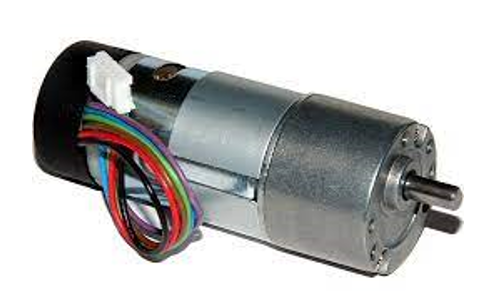
\includegraphics[width=0.6\textwidth]{motorEMG30}
	\caption{Motor EMG30 utilizado en la planta piloto.}
\end{figure}
\FloatBarrier

Es ideal para aplicaciones robóticas pequeñas o medianas. También incluye un condensador de supresión de ruido estándar en el motor. Las conexiones del motor son:

\begin{enumerate}
\item Purple (1) Hall Sensor B Vout
\item Blue (2) Hall sensor A Vout
\item Green (3) Hall sensor ground
\item Brown (4) Hall sensor Vcc
\item Red (5) + Motor
\item Black (6) - Motor
\end{enumerate}

Estas conexiones van conectadas a la placa que se muestra en la Figura \ref{controlMotor} y será la encargada de controlar los bytes recibidos y enviados.

%\imagen{placaMotor}{Placa controladora de los motores} \label{controlMotor}
\begin{figure}[!h]
	\centering
	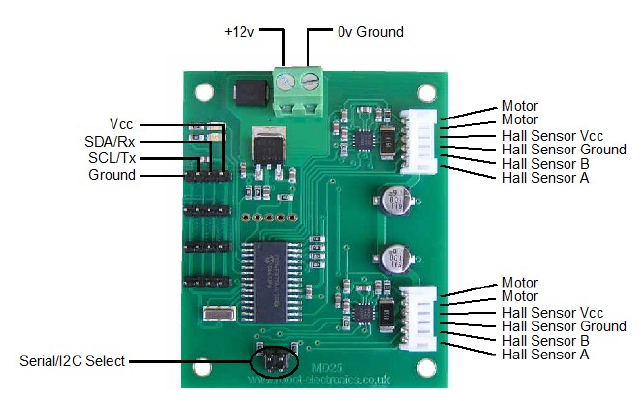
\includegraphics[width=0.9\textwidth]{placaMotor}
	\caption{Placa controladora de los motores.}\label{controlMotor}
\end{figure}

La placa K64F envía a través de conexión UART o I2C los bytes con las instrucciones para los motores a la placa controladora y posteriormente esta placa enviará la información al propio motor que realizará las acciones correspondientes a ese comando. 
Por otro lado, los bytes enviados consisten, en la mayoría de las instrucciones, en un byte de sincronización, un byte para elegir el motor, puesto que se pueden conectar hasta dos motores, y el byte con la instrucción. Estos bytes se pueden enviar tanto en formato hexadecimal como decimal u octal.
Vamos a ver los modos y comandos que se pueden utilizar con estos motores.
En cuanto a los modos disponemos de 4 modos:
\begin{itemize}
\item Modo 0. Si se elegimos usar el modo 0 entonces los registros de velocidad son velocidades literales en el rango de 0 (retroceso total)
128 (parada) 255 (avance total).
\item Modo 1. El modo 1 es similar al modo 0, excepto que los valores de velocidad se interpretan como valores con signo. El rango es -128
(retroceso total) 0 (parada) 127 (avance total).
\item Modo 2. En el modo 2 la velocidad 1 controle la velocidad de ambos motores, y la velocidad2 se convierte en el valor de giro. Los datos están en el rango de 0 (retroceso total) 128 (parada) 255 (avance total).
\item Modo 3. El modo 3 es similar al modo 2, excepto que los valores de velocidad se interpretan como valores con signo. Los datos están en el rango de -128 (retroceso total) 0 (parada) 127 (avance total).
\end{itemize}

En la Tabla \ref{tabla:ComandosMotores} se muestran los comandos (CMD) más importantes y su descripción.

\tablaSmallSinColores{Comandos Motores EMG30.}{l c c l}{ComandosMotores}
{\multicolumn{1}{c}{ CMD } & Nombre & Bytes & Descripción\\ 
 & & Env-Rec & \\}
{
0x21 & Get Speed 1 & 2 - 1 & Obtener la velocidad del motor A\\
0x22 & Get Speed 1 & 2 - 1 & Obtener la velocidad del motor B\\
0x2A & Get Acceleration & 2 - 1 & Devuelve la aceleración\\
0x31 & Set Speed 1 & 3 - 0 & Fija la velocidad del motor A\\
0x32 & Set Speed 1 & 3 - 0 & Fija la velocidad del motor B\\
0x33 & Set Acceleration & 3 - 0 & Fija la aceleración\\
0x34 & Set Mode & 3 - 0 & Fija el modo\\ 
0x38 & TimeOut OFF & 2 - 0 & No apagar en 2s sin comunicación\\
0x39 & TimeOut ON & 2 - 0 & Apagar tras 2s sin comunicación\\
}

\subsection{Sensor de Temperatura: LM35}

\begin{figure}[!h]
	\centering
	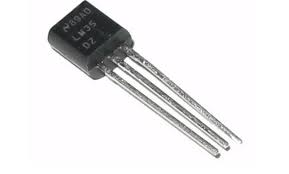
\includegraphics[width=0.6\textwidth]{Tmp}
	\caption{Sensor de temperatura, LM35.}
\end{figure}
\FloatBarrier

El sensor de temperatura LM35, es un circuito electrónico cuyas características se describieron en el capitulo anterior \ref{potenySensorTemp}, de salida analógica, que permite medir temperaturas. Este sensor proporciona un voltaje proporcional a la temperatura en la que se encuentra. Tiene un rango de medición desde -55 grados centígrados, hasta un máximo de 150 grados.
Sus características principales son:
\begin{itemize}
\item Resolución: 10mV por grado centígrado.
\item Voltaje de alimentación.  Por ejemplo, este sensor se puede alimentar desde 4Vdc hasta 20Vdc.
\item Tipo de medición: Salida analógica.
\item Numero de pines: 3 pines, GND, VCC y VSalida.
\end{itemize}


\subsection{Wifi: módulo ESP8266}

El módulo ESP8266 \cite{moduloEsp8266} se trata de un chip integrado con conexión Wifi y compatible con el protocolo TCP/IP. El objetivo principal es dar acceso a cualquier microcontrolador a una red. La gran ventaja del ESP8266 es su bajo consumo. Soporta IPv4 y los protocolos TCP/UDP/HTTP/FTP. La Figura \ref{pinesESP} muestra los pines del módulo ESP8266.

%\imagen{pines8266}{Pines del módulo wifi 8266}  \label{pinesESP}
\begin{figure}[!h]
	\centering
	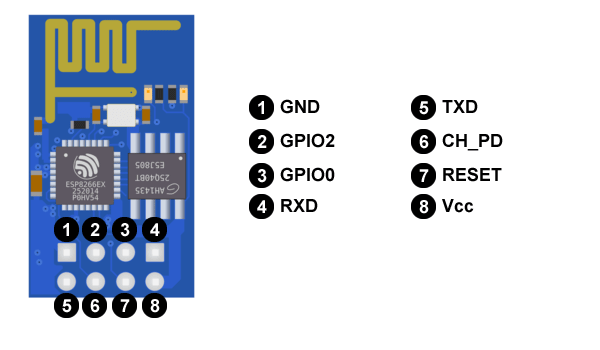
\includegraphics[width=0.9\textwidth]{pines8266}
	\caption{Pines del módulo wifi 8266.}\label{pinesESP}
\end{figure}

\textbf{ESP32 soporta las siguientes características:}
\begin{itemize}
\item Soporta los principales buses de comunicación (SPI, I2C, UART).
\item Comunicación unicast encriptada y sin encriptar.
\item Se pueden mezclar clientes con encriptación y sin encriptación.
\item Permite enviar hasta 250 bytes de carga útil.
\item Se pueden configurar \extranjerismo{callbacks} para informar a la aplicación si la transmisión fue correcta.
\item Largo alcance, pudiendo superar los 200 metros en campo abierto.
\end{itemize}

\textbf{Pero también tiene sus limitaciones:}
\begin{itemize}
\item El número de clientes con encriptación está limitado. Esta limitación es de 10 clientes para el modo Estación, 6 como mucho en modo punto de acceso o modo mixto.
\item El número total de clientes con y sin encriptación es de 20.
\item Sólo se pueden enviar hasta 250 bytes.
\end{itemize}

\subsubsection{Uso del módulo ESP8266}
El módulo ESP8266 \cite{tutorialESP} es un dispositivo TTL ``Serial to Wireless Internet'' funciona mediante el envío de comandos `AT'. En la Tabla \ref{tabla:ComandosAT} se explican los comandos más importantes. Los comandos están ordenados según los pasos que se deberían seguir para establecer comunicación entre un módulo y un servidor.

\clearpage

\tablaSmallSinColores{Comandos AT.}{l l}{ComandosAT}
{\multicolumn{1}{c}{Comando} & Descripción\\}
{
AT+CWMODE=`X' & \parbox{.5\textwidth}{\begin{itemize}
  	\item 1 = Modo estación (cliente)
	\item 2 = Modo AP (huésped)
	\item 3 = Modo AP + Estación (modo dual)
    \end{itemize}}\\ \hline \\
AT+CWLAP & Lista APs disponibles \\ \hline \\
AT+CWJAP=`ssid',`Pswd' & \parbox{.5\textwidth}{El módulo se conecta a la red con el nombre ssid indicado y la contraseña pwd suministrada.} \\ \hline \\
AT+CIPMUX=`X' & \parbox{.5\textwidth}{\begin{itemize}
  	\item 0 = Conexión única
	\item 1 = Múltiples conexiones, hasta 4
    \end{itemize}}\\ \hline \\
AT+CIPSERVER=Mode,puerto & \parbox{.5\textwidth}{
Configura el módulo como servidor donde el
modo:	
	\begin{itemize}
  	\item 0 = Borrar servidor
	\item 1 = Crear servidor
    \end{itemize}
    puerto: número del puerto, por defecto es el 333}\\ \hline \\
AT+CIFSR & \parbox{.5\textwidth}{Retorna la dirección IP local del módulo como cliente.} \\ \hline \\
AT+CIPSEND & \parbox{.5\textwidth}{Envía datos sin adornos cada 20ms. El módulo retorna ">" después ejecutar el comando, si se recibe el comando "+++" se regresa al modo comando.}\\
}

\section{Herramientas software}\label{sec:HSoftware}

Veamos que herramientas software he utilizado a lo largo del desarrollo del proyecto.

\begin{description}
\item[KDS IDE.]
Kinetis ® Design Studio (KDS) es un entorno de desarrollo integrado complementario para los MCU Kinetis que permite una edición, compilación y depuración sólidas de sus diseños.
Kinetis está basado en software gratuito de código abierto que incluye Eclipse, GNU Compiler Collection (GCC), GNU Debugger (GDB) y otros, Kinetis Design Studio IDE ofrece a los diseñadores una herramienta de desarrollo simple sin limitaciones de tamaño de código. 
Además, el software Processor Expert ® habilita su diseño con su base de conocimiento y ayuda a crear aplicaciones potentes con unos pocos clics.

Este fue el IDE sobre el que empecé el proyecto y del que tras un par de semanas terminaría migrando a MCUXPRESSO 
Entorno multiplataforma basado en software libre como Eclipse IDE o GNU Compiler Collection (GCC). Incorpora Processor Expert, una utilidad que permite añadir y configurar los componentes necesarios para un proyecto.


\item[MCUXpresso IDE.]
Este IDE está basado en eclipse y sobre el que se ha desarrollado el proyecto. 
El IDE de MCUXpresso \cite{MCUXDownload} ofrece funciones avanzadas de edición, compilación y depuración. Añade también vistas de depuración específicas de MCU, rastreo y creación de perfiles de código, además de depuración multinúcleo y herramientas de configuración integradas. Es un IDE muy completo que presenta una interfaz simple para el usuario pese a gran número de opciones y configuraciones que ofrece.

\section{FreeRTOS}\label{sec:RTOS}
Algunos apartados más atrás ya hablamos sobre que era un \extranjerismo{RTOS} \ref{ref:SOTiempoReal}, en esta sección veremos cual ha sido el sistema operativo que he utilizado en este proyecto. \\
FreeRTOS \cite{web:FreeRtos} es robusto, tiene un tamaño reducido y  una compatibilidad del 100\% con el microcontrolador. Es el sistema operativo en tiempo real más utilizado en microcontroladores pequeños en el mundo.\\
Además cuenta con varias demostraciones preconfiguradas y detalladas referentes al Internet de las cosas (IoT). AWS se encarga de su mantenimiento y soporte a largo plazo.
Como hemos podido observar es un software completísimo, referente mundial, fácil de usar y con un soporte que saca actualizaciones constantemente.


\subsection{LwIP}
La librería light weight IP pretende dar un servicio basado en el protocolo TCP/IP. Este software fue desarrollado por Adam Dunkels en Computer and Laboratory de Arquitecturas de Redes (CNA) en el Instituto Sueco de Ciencias de la Computación (SICS).

El enfoque de la implementación de lwIP TCP/IP es reducir el uso de RAM sin dejar de tener un TCP a escala completa. Esto hace que lwIP sea adecuado para su uso en sistemas embebidos con decenas de kilobytes de RAM libre y espacio para alrededor de 40 kilobytes de código ROM.

\subparagraph{Protocolos implementados}
\begin{itemize}
  \item IP (Protocolo de Internet, IPv4 e IPv6), incluido el reenvío de paquetes múltiples interfaces de red.
  \item ICMP (Protocolo de mensajes de control de Internet) para mantenimiento y depuración de redes.
  \item IGMP (Protocolo de gestión de grupos de Internet) para la gestión del tráfico de multidifusión.
  \item MLD (descubrimiento de oyentes de multidifusión para IPv6). Tiene como objetivo cumplir con RFC 2710. Sin soporte para MLDv2.
  \item ND (descubrimiento de vecinos y configuración automática de direcciones sin estado para IPv6).
    Tiene como objetivo cumplir con RFC 4861 (descubrimiento de vecinos) y RFC 4862
    (Autoconfiguración de direcciones).
  \item UDP (Protocolo de datagramas de usuario) que incluye extensiones UDP-lite experimentales.
  \item TCP (Protocolo de control de transmisión) con control de congestión, estimación de RTT y recuperación rápida/retransmisión rápida.
  \item API nativa/sin formato para un rendimiento mejorado.
  \item API de socket similar a Berkeley opcional.
  \item DNS (resolución de nombres de dominio).
\end{itemize}

\item[Dockligth.]
Docklight \cite{DocklightDownload} es una herramienta de prueba, análisis y simulación de protocolos de comunicación en serie.
Este programa se utiliza para captar las comunicaciones serie y Uart. En este proyecto se ha utilizado para poder comunicarnos con la placa de una manera más sencilla a la hora de tener que introducir comandos. Para la captura de estos mensajes es necesario conocer el puerto de salida 'comm' y la velocidad en baudios a la que se transmiten los datos, además del número de bits, paridad, etc.
Por otro lado, este software cuenta con algunas características añadidas como poder guardar comandos que usamos de forma continua o poder ver la información en ascii, binario o hexadecimal que en algunas ocasiones puede ser necesario.

\item[Termite.]
Este software es muy parecido a Docklight pero en este caso cuenta con una interfaz más simple. En este caso el programa se configura con los parámetros del otro dispositivo con el que nos vamos a comunicar y se reciben o envían datos.

\item[Packet Sender.]
Este programa ha sido de gran ayuda puesto que se utilizó para realizar las pruebas de recepción y envío de paquetes a las tres placas. 
Packet Sender es una utilidad de código abierto que permite enviar y recibir paquetes TCP y UDP. También admite conexiones TCP mediante SSL, generación de tráfico intenso, solicitudes HTTP GET/POST y generación de paneles.
\end{description}


\section{Herramientas de documentación}\label{sec:HDocumentacion}
Veamos las herramientas utilizadas para documentar y trabajar sobre el proyecto.

\begin{description}
\item[Textmaker. \cite{wiki:TextMaker}]
Es una herramienta gratuita que nos ayuda a escribir documentos de texto integrando las funciones necesarias para poder realizar documentos con Latex. Además este software es multiplataforma.
\item[Latex. \cite{wiki:latex}]
Latex es un compositor de textos destinado a la creación de documentos profesionales que requieran una alta calidad tipográfica. Se utiliza, por lo general, en la realización de artículos y libros científicos que incluyen elementos y expresiones matemáticas.
\item[Bibtex. \cite{bibtex}]
Es una herramienta utilizada para la creación de referencias bibliográficas. Genera un formato para cada una de las referencias con los datos aportados por el usuario y generalmente se utiliza en la realización de documentos con LaTeX.
\end{description}

\section{Herramientas de comunicación}\label{sec:HComunicacion}
Para la comunicación con mis tutores para aclarar dudas y resolver fallos se han utilizado las siguientes herramientas.

\begin{description}
\item[Microsoft Outlook. \cite{wikiOutlook}] Es un gestor de correo electrónico desarrollado por Microsoft y que podemos encontrar en la suite de Microsoft office.

\item[Microsoft Teams. \cite{wikiTeams}] De nuevo es un programa desarrollado por Microsoft. En este caso se trata de una plataforma para realizar reuniones virtuales, cuenta también con salas de chat y la posibilidad de generar documentos compartidos.
\end{description}


\section{Herramientas de gestión de proyectos}\label{sec:HGestionProyectos}
En el primer apartado hablábamos de la técnica de organización y desarrollo de proyectos mediante metodologías ágiles: SCRUM, en este apartado veremos cuales son las herramientas con las que conseguimos facilitar estas tareas.

\begin{description}
\item[GitHub. \cite{GitHub}]
GitHub es una plataforma pensada para que los desarrolladores puedan alojar su repositorios de código de forma segura en la nube. Además incluye un sistema de control de versiones conocido como Git. \\
Por otro lado, también permite el desarrollo colaborativo entre distintos desarrolladores y ofrece todas las herramientas para poder trabajar con SCRUM. 

\item[GitKraken. \cite{GitKraken}]
GitKraken es una aplicación que nos permite manejar Git y por tanto nuestros archivos de GitHub de forma más sencilla. Esta herramienta se encuentra disponible para todas las plataformas.
\end{description}









